% Chapter Template

\chapter{Comments-Observations} % Main chapter title

\label{Chapter7}

Concluding the internship's report, I would like to make some comments regarding:

\begin{itemize}

	\item my working environment and my team: the company is structured based on Agile methodologies and is human oriented providing to its employees the equipment and the supplies needed.
	\item the team I was a part of: my team was investing time in bounding and collaborating with each other. One of the main principles was to support each other in timed of need.
	\item the factors which created obstacles or difficulties in my work: The organization employs a large number of people which is separated in various groups. These groups are hosted in different building owned by the company, which is something that causes long processing in getting access to different projects. 
	\item the factors which helped me to carry out the activities requested: my colleagues' and especially my supervisor's contribution was essential to what I have achieved. The one to one meetings we had, helped me improve my skills in coding and learn the way the procedures were executed inside the team.
	\item the knowledge / experience I gained: Regarding what I have learned through this experience, I gained skills and knowledge in ReactJS, JavaScript, Node.js, creation of npm packages, and generally how to work in a team, as well as how to display code that will be deployed.
	\item proposals to improve the department's functionality: As I have already mentioned, one of the main difficulties in my work environment is the long processing in getting access to different projects. This is because of the company's structure. Therefore, I would suggest restructuring the faculties and minimizing the complexity of them.
\end{itemize}


\chapter{Appendix}

\section{Stas NPM package - ReadME.md file}
	\textbf{Install}
	
	\begin{lstlisting}[language=bash]
	$ npm install @freenow-gr/stats$
	\end{lstlisting}
	
	or
	
	\begin{lstlisting}[language=bash]
	$ yarn add @freenow-gr/stats$
	\end{lstlisting}

	\textbf{Usage}
	
	\begin{lstlisting}[language=JavaScript]
	import {groupStatistics, KPI, resolutions} 
			from "@freenow-gr/stats";
	
	const validMockedData = {
		y2019: {
			m3: {
				d12: {
					h15: {
						CancelledCounter: 1,
						CompletedCounter: 3,
						revenueSum: 258.47,
					},
				},
			},
		},
	};	
	const args = {
		statsObject:validMockedData, 
		startTimestamp: new Date('2018-02-10T15:45:00'), 
		endTimestamp: new Date('2018-02-12T15:45:00'), 
		kpi:KPI.GMV, 
		resolution:resolutions.HOUR
	}
	\end{lstlisting}
	
	\newpage
	In order to run you need to have an object like this:
	
	\begin{lstlisting}[language=JavaScript]
	let result = groupStatistics(args);
	console.log(result);
	//y2018: {
	//	m2: {
	//		d12: {
	//			h15: {
	//				revenueSum: 258.47,
	//				},
	//			},
	//		},
	//	}
	
	\end{lstlisting}
	
	
\section{Landing Page - Responsive in all devices}

The landing page created for mpaineis-vgaineis competition was used from a large amount of Beat and non-Beat users. The page had to be responsive and differently displayed in a variety of mobiles, tablets and desktops, and also to match with the designs given through Zeplin and shown in figure 8.1.

\begin{figure}[H]
	\begin{center}
		
\includegraphics[scale=0.4]{images/my_projects/landing_page/zeplin.png}
	\end{center}
	\caption{Designs of Landing page in Zeplin}
\end{figure}

Following, it is presented every screen on a mobile device, taken from \url{mpaineis-vgaineis.gr}. The same screens in desktop exist in figures 4.4 and 4.5 of Chapter \ref{Chapter5}.
\begin{figure}[H]
	\centering
	\subfloat{{
\includegraphics[scale=0.18]{images/my_projects/landing_page/header-mobile.jpg} }}%
	\qquad
	\subfloat{{
\includegraphics[scale=0.18]{images/my_projects/landing_page/description-mobile.png} }}%
	\qquad
	\subfloat{{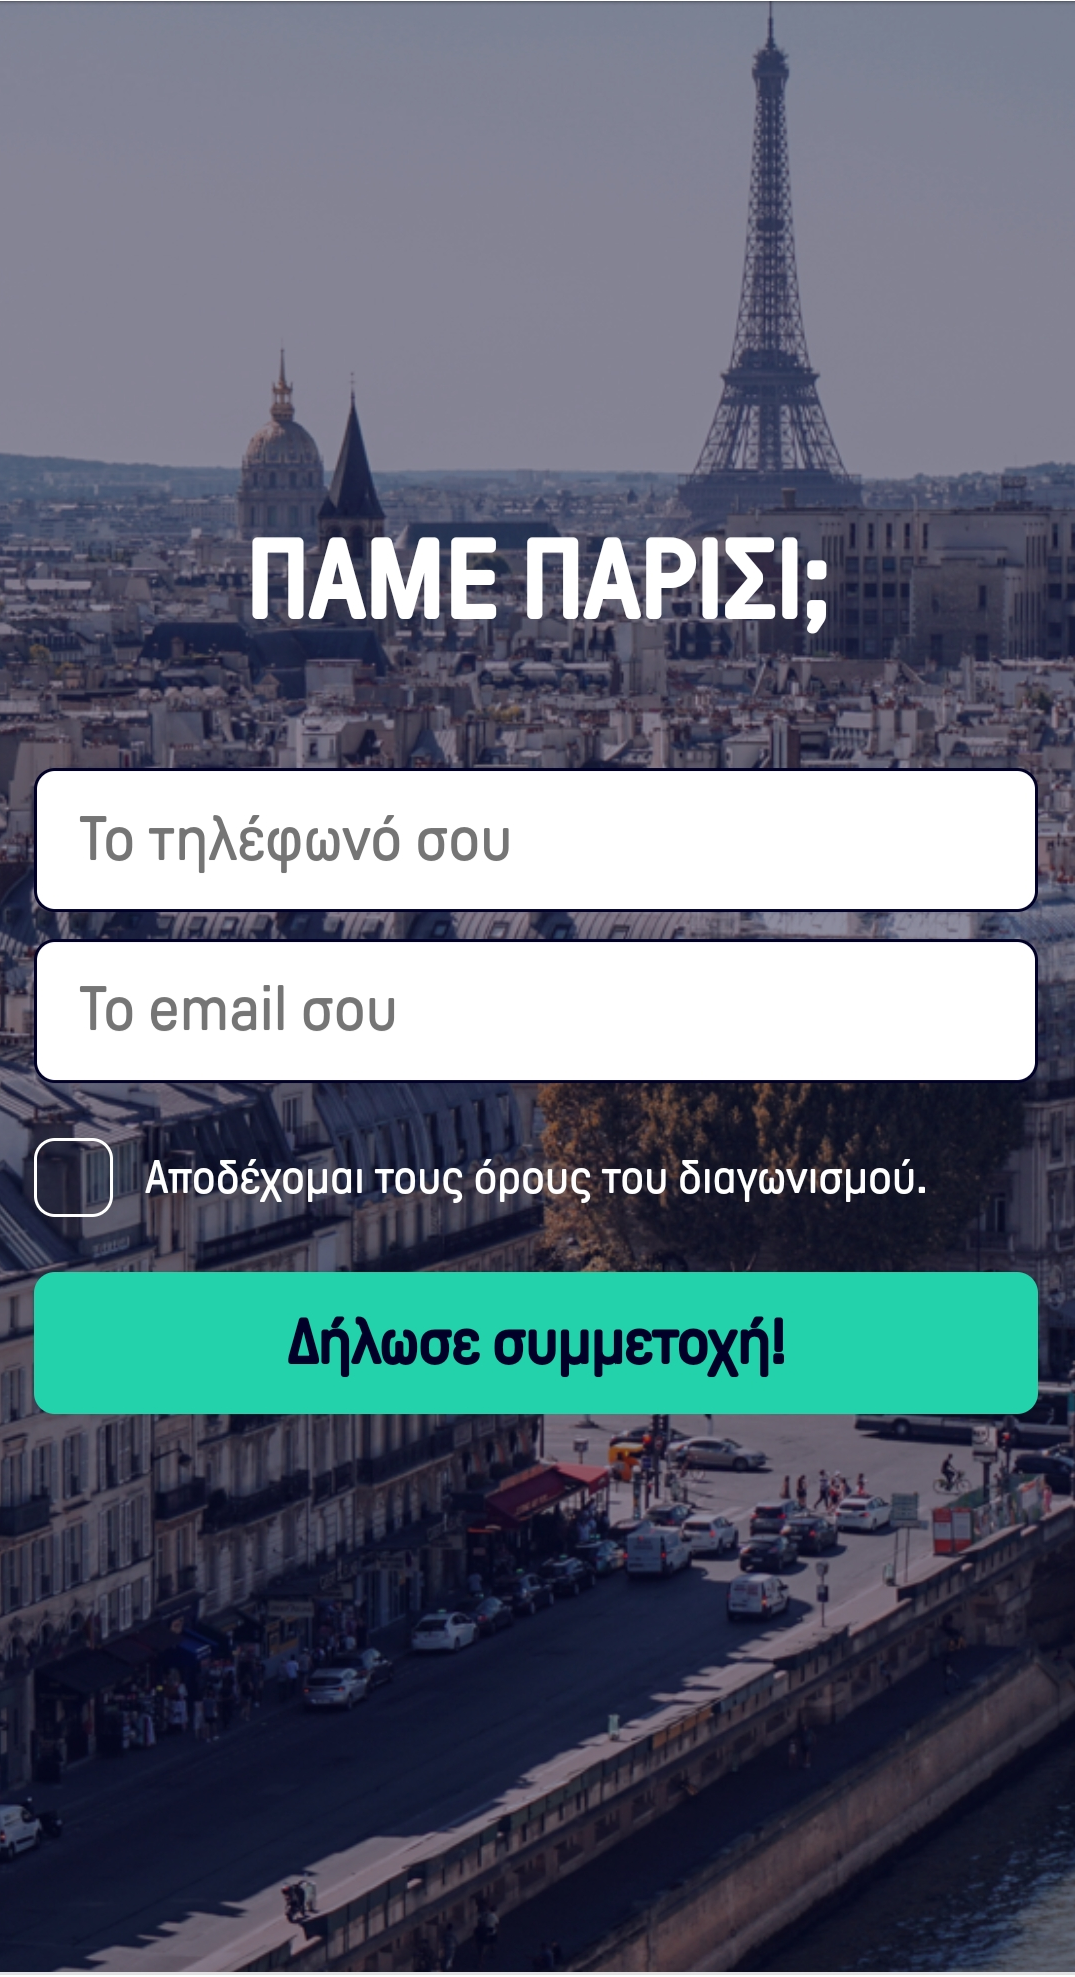
\includegraphics[scale=0.18]{images/my_projects/landing_page/form-mobile.png} }}%
	\caption{
		Landing Page for Competition mpaineis-vgaineis
		\\
		\textbf{Online: } \url{https://mpaineis-vgaineis.gr/}
	}
	\label{fig:example}
\end{figure}

\begin{figure}[H]
	\centering
	\subfloat{{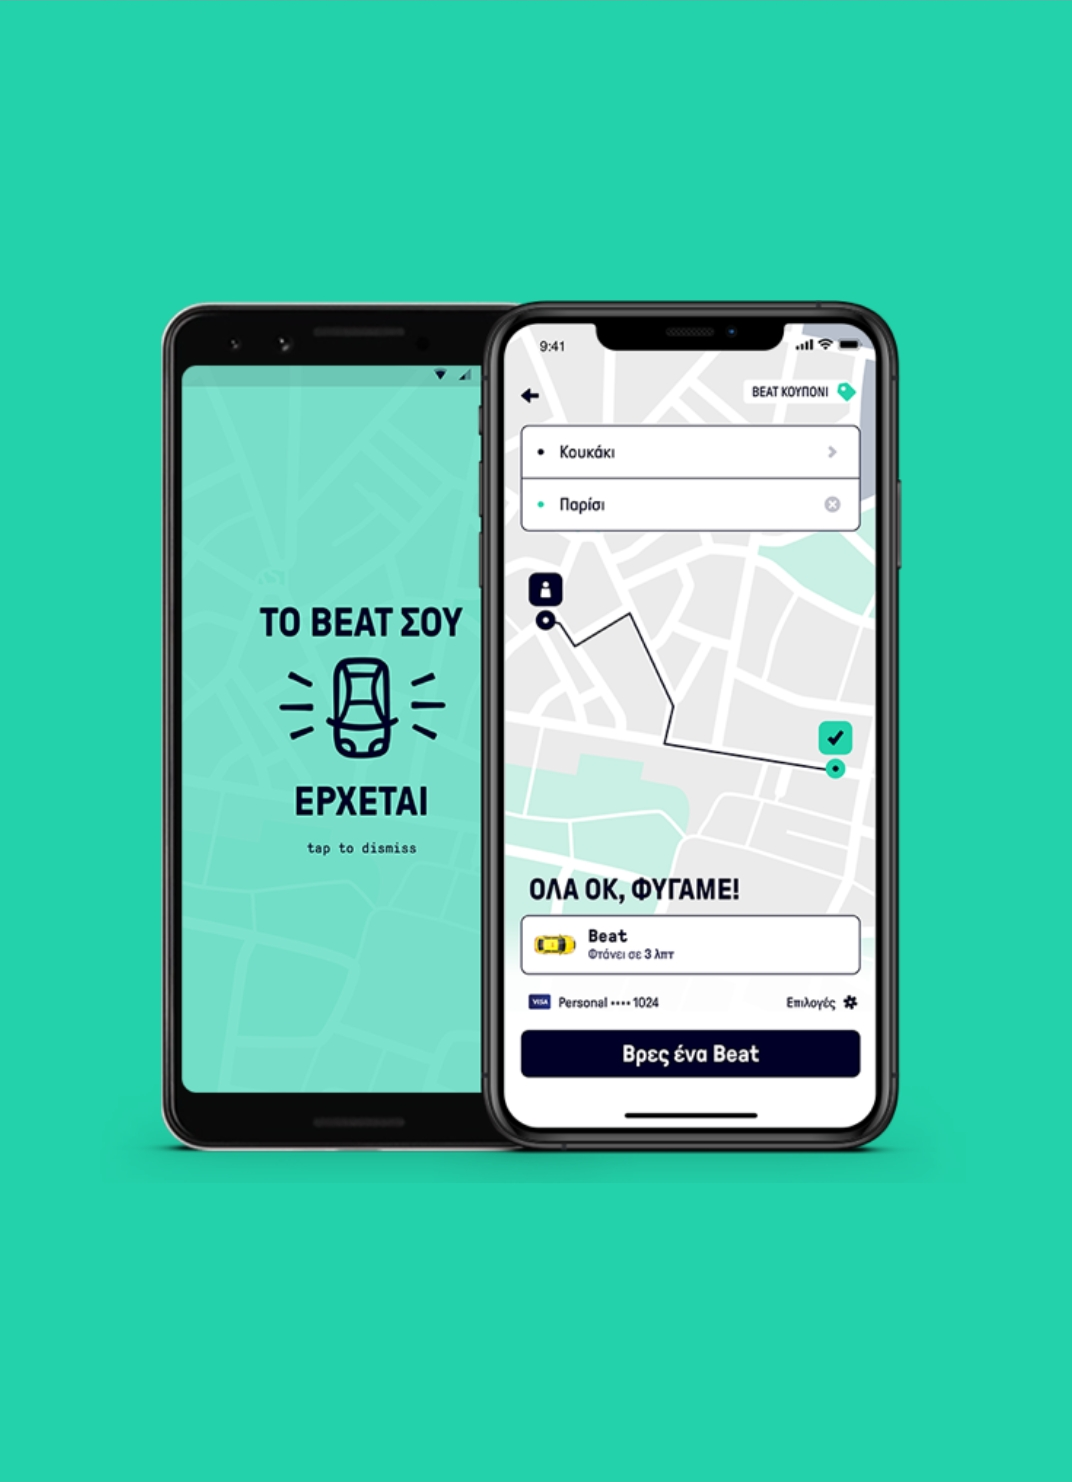
\includegraphics[scale=0.18]{images/my_projects/landing_page/app-mobile.png} }}%
	\qquad
	\subfloat{{
\includegraphics[scale=0.18]{images/my_projects/landing_page/app-download-mobile.png} }}%
	\qquad
	\subfloat{{
\includegraphics[scale=0.18]{images/my_projects/landing_page/footer-mobile.png} }}%
	\caption{
		Landing Page for Competition mpaineis-vgaineis
		\\
		\textbf{Online: } \url{https://mpaineis-vgaineis.gr/}
	}
	\label{fig:example}
\end{figure}

\begin{figure}[H]
	\centering
	\subfloat{{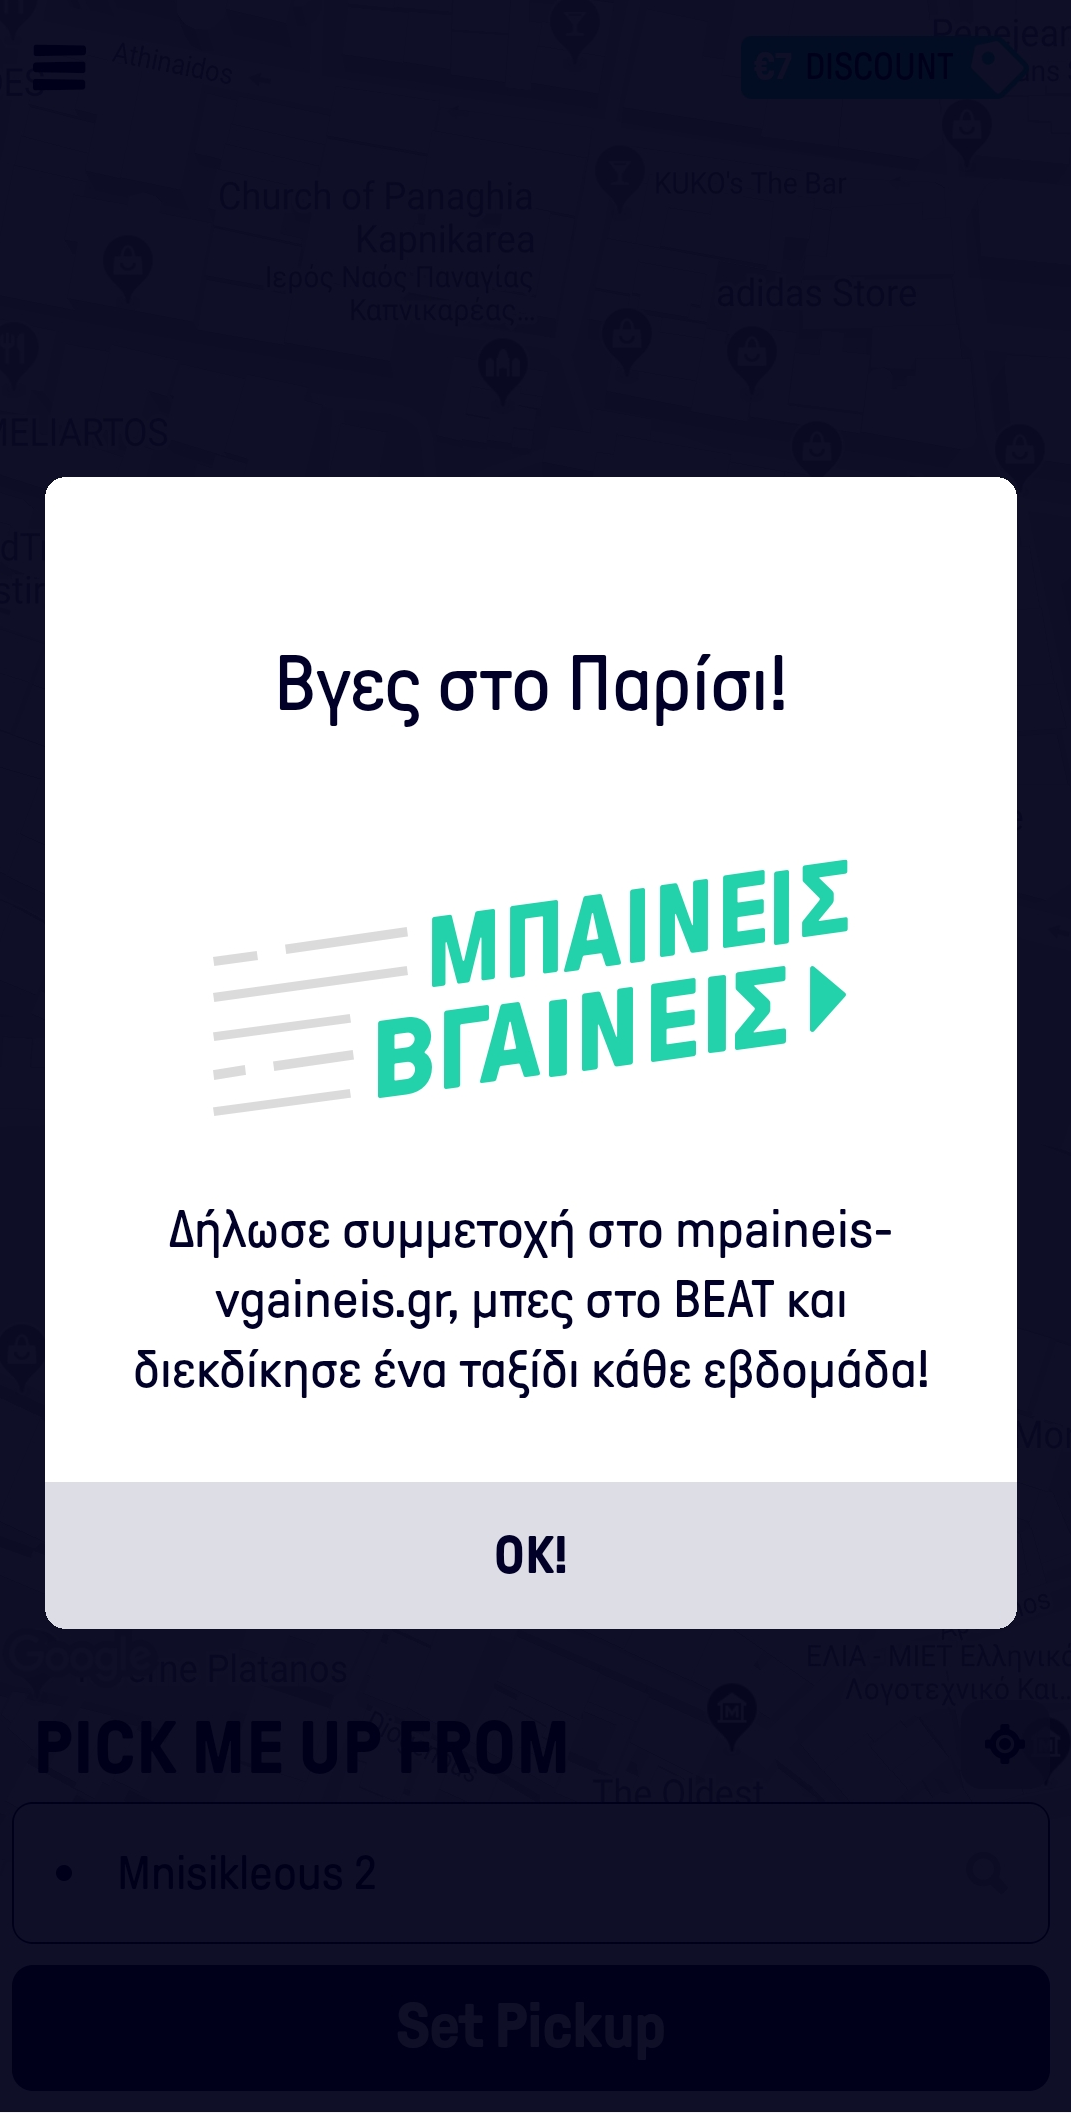
\includegraphics[scale=0.2]{images/my_projects/landing_page/popup-confirmation-mobile.png} }}%
	\qquad
	\subfloat{{
\includegraphics[scale=0.2]{images/my_projects/landing_page/limits-mobile.png} }}%
	\caption{
		Landing Page for Competition mpaineis-vgaineis
		\\
		\textbf{Online: } \url{https://mpaineis-vgaineis.gr/}
	}
	\label{fig:example}
\end{figure}

\section{Geo Npm Package - ReadME.md file}

\textbf{Install}

\begin{lstlisting}[language=bash]
$ npm install @freenow-gr/geo
\end{lstlisting}

or
\begin{lstlisting}[language=bash]
$ yarn add @freenow-gr/geo
\end{lstlisting}

\textbf{Usage}

\begin{lstlisting}[language=JavaScript]
const getDistance = require("@freenow-gr/geo");

rideDetails = {
	"1553975075880": {
		"accuracy": 15.080751419067383,
		"heading": 52.33772277832031,
		"latitude": 37.963367633154164,
		"longitude": 23.722526298787404,
		"speed": 6.180961608886719
	},
	"1553975130608": {
		"accuracy": 4.900000095367432,
		"heading": 130.42340087890625,
		"latitude": 37.964163783535504,
		"longitude": 23.723863186483126,
		"speed": 0
	},
	"1553975187680": {
		"accuracy": 4.900000095367432,
		"heading": 80.70649719238281,
		"latitude": 37.96529748280323,
		"longitude": 23.725764682563828
	}
}

rideDetailsWrongKeys = {
	"1553975075880": {
		"accuracy": 15.080751419067383,
		"heading": 52.33772277832031,
		"speed": 6.180961608886719
	},
	"1553975130608": {
		"accuracy": 4.900000095367432,
		"heading": 130.42340087890625,
		"Latitude": 37.964163783535504, // needs to be in lowercase
		"wrongLongitude": 23.723863186483126,
		"speed": 0
	}
}

rideDetailsWrongValues = {
	"1553975075880": {
		"accuracy": 15.080751419067383,
		"heading": 52.33772277832031,
		"latitude": "notNumber",
		"longitude": 23.722526298787404,
		"speed": 6.180961608886719
	},
	"1553975130608": {
		"accuracy": 4.900000095367432,
		"heading": "130.42340087890625", // string, not a number
		"latitude": 37.964163783535504,
		"longitude": 23.723863186483126,
		"speed": 0
	}
}

result = getDistance(rideDetails);
console.log(result);
// => 0.3558715732059
// result is km

result = getDistance(123);
console.log(result);
// => 0

result = getDistance(rideDetailsWrongKeys);
console.log(result);
// => Wrong key name of input. 
		There are no latitude, longitude as keys.

result = getDistance(rideDetailsWrongValues);
console.log(result);
// => Wrong values of keys latitude, longitude. 
		Their values need to be numbers.
\end{lstlisting}
